%%%%%%%% ICML 2026 EXAMPLE LATEX SUBMISSION FILE %%%%%%%%%%%%%%%%%

\documentclass{article}

% Recommended, but optional, packages for figures and better typesetting:
\usepackage{microtype}
\usepackage{graphicx}
\usepackage{subcaption}
\usepackage{booktabs} % for professional tables

% hyperref makes hyperlinks in the resulting PDF.
% If your build breaks (sometimes temporarily if a hyperlink spans a page)
% please comment out the following usepackage line and replace
% \usepackage{icml2026} with \usepackage[nohyperref]{icml2026} above.
\usepackage{hyperref}


% Attempt to make hyperref and algorithmic work together better:
\newcommand{\theHalgorithm}{\arabic{algorithm}}

% Use the following line for the initial blind version submitted for review:
\usepackage{icml2026}

% For preprint, use
% \usepackage[preprint]{icml2026}

% If accepted, instead use the following line for the camera-ready submission:
% \usepackage[accepted]{icml2026}

\usepackage{amsmath}
\usepackage{amssymb}
\usepackage{mathtools}
\usepackage{amsthm}


% if you use cleveref..
\usepackage[capitalize,noabbrev]{cleveref}

% ---- Packages ----
\usepackage{microtype}
\usepackage{graphicx}
\usepackage{subcaption}
\usepackage{booktabs}
\usepackage{multirow}
\usepackage{amsmath, amssymb, amsfonts}
\usepackage{mathtools}
\usepackage{bm}
\usepackage{algorithm}
\usepackage{algorithmic}
\usepackage{hyperref}
\usepackage{cleveref}
% \usepackage{enumitem}
\usepackage[inline, shortlabels]{enumitem}
\usepackage{xcolor}
\usepackage{amsthm}

% ---- Optional: TikZ for figures ----
\usepackage{tikz}
\usetikzlibrary{positioning, arrows.meta, calc}

% ---- Handy commands (edit later) ----
\newcommand{\wm}{\textsc{WM}}
\newcommand{\mawm}{\textsc{MAWM}}
\newcommand{\nsm}{\textsc{NS-MAWM}}
\newcommand{\DecPOMDP}{\textsc{Dec-POMDP}}
\newcommand{\RVR}{\textsc{RVR}}
\newcommand{\KL}{\mathrm{KL}}

% Spell-checker exceptions for acronyms and domain-specific terms
% \usepackage{spellcheck}
% \spellcheck{MAWM,NS-MAWM,gridworld,SMAC,neuro-symbolic}

% --- Tickz
\usepackage{physics}
\usepackage{tikz}
\usetikzlibrary{arrows.meta,positioning,fit,calc}
\usepackage{amsmath}
\usepackage{mathdots}
% \usepackage{yhmath}
\usepackage{cancel}
\usepackage{color}
\usepackage{siunitx}
\usepackage{array}
\usepackage{multirow}
% \usepackage{amssymb}
\usepackage{gensymb}
\usepackage{tabularx}
\usepackage{extarrows}
\usepackage{booktabs}
\usetikzlibrary{fadings}
\usetikzlibrary{patterns}
\usetikzlibrary{shadows.blur}
\usetikzlibrary{shapes}

% ---- Math shortcuts ----
\newcommand{\E}{\mathbb{E}}
\newcommand{\R}{\mathbb{R}}
\newcommand{\I}{\mathbb{I}}

\usepackage{amssymb}
\usepackage{pifont}

\newcommand{\cmark}{\ding{51}}%
\newcommand{\xmark}{\ding{55}}%

\usepackage[english]{babel}
\addto\extrasenglish{  
    \def\figureautorefname{Figure}
    \def\tableautorefname{Table}
    \def\algorithmautorefname{Algorithm}
    \def\sectionautorefname{Section}
    \def\subsectionautorefname{Subsection}
    \def\proofoutlineautorefname{Proof Outline}
}

%%%%%%%%%%%%%%%%%%%%%%%%%%%%%%%%
% THEOREMS
%%%%%%%%%%%%%%%%%%%%%%%%%%%%%%%%
\theoremstyle{plain}
\newtheorem{theorem}{Theorem}[section]
\newtheorem{proposition}[theorem]{Proposition}
\newtheorem{lemma}[theorem]{Lemma}
\newtheorem{corollary}[theorem]{Corollary}
\theoremstyle{definition}
\newtheorem{definition}[theorem]{Definition}
\newtheorem{assumption}[theorem]{Assumption}
\theoremstyle{remark}
\newtheorem{remark}[theorem]{Remark}

% Todonotes is useful during development; simply uncomment the next line
%    and comment out the line below the next line to turn off comments
%\usepackage[disable,textsize=tiny]{todonotes}
\usepackage[textsize=tiny]{todonotes}

% The \icmltitle you define below is probably too long as a header.
% Therefore, a short form for the running title is supplied here:
\icmltitlerunning{Neuro-Symbolic Multi-Agent World Models}

\begin{document}

\twocolumn[
  \icmltitle{Invariant-Aware Neuro-Symbolic Multi-Agent World Models\\
    for Model-Based Multi-Agent Reinforcement Learning}

  % It is OKAY to include author information, even for blind submissions: the
  % style file will automatically remove it for you unless you've provided
  % the [accepted] option to the icml2026 package.

  % List of affiliations: The first argument should be a (short) identifier you
  % will use later to specify author affiliations Academic affiliations
  % should list Department, University, City, Region, Country Industry
  % affiliations should list Company, City, Region, Country

  % You can specify symbols, otherwise they are numbered in order. Ideally, you
  % should not use this facility. Affiliations will be numbered in order of
  % appearance and this is the preferred way.
  \icmlsetsymbol{equal}{*}

  \begin{icmlauthorlist}
    \icmlauthor{Julien Soulé}{equal,yyy}
    \icmlauthor{Georgios Bakirtzis}{equal,yyy,comp}
    \icmlauthor{Jean-Paul Jamont}{comp}
    \icmlauthor{Firstname4 Lastname4}{sch}
    \icmlauthor{Firstname5 Lastname5}{yyy}
    \icmlauthor{Firstname6 Lastname6}{sch,yyy,comp}
    \icmlauthor{Firstname7 Lastname7}{comp}
    %\icmlauthor{}{sch}
    \icmlauthor{Firstname8 Lastname8}{sch}
    \icmlauthor{Firstname8 Lastname8}{yyy,comp}
    %\icmlauthor{}{sch}
    %\icmlauthor{}{sch}
  \end{icmlauthorlist}

  \icmlaffiliation{yyy}{Department of XXX, University of YYY, Location, Country}
  \icmlaffiliation{comp}{Company Name, Location, Country}
  \icmlaffiliation{sch}{School of ZZZ, Institute of WWW, Location, Country}

  \icmlcorrespondingauthor{Julien Soulé}{julien.soule@hotmail.fr}
  \icmlcorrespondingauthor{Firstname2 Lastname2}{first2.last2@www.uk}

  % You may provide any keywords that you find helpful for describing your
  % paper; these are used to populate the "keywords" metadata in the PDF but
  % will not be shown in the document
  \icmlkeywords{Machine Learning, ICML}

  \vskip 0.3in
]

% this must go after the closing bracket ] following \twocolumn[ ...

% This command actually creates the footnote in the first column listing the
% affiliations and the copyright notice. The command takes one argument, which
% is text to display at the start of the footnote. The \icmlEqualContribution
% command is standard text for equal contribution. Remove it (just {}) if you
% do not need this facility.

% Use ONE of the following lines. DO NOT remove the command.
% If you have no special notice, KEEP empty braces:
\printAffiliationsAndNotice{}  % no special notice (required even if empty)
% Or, if applicable, use the standard equal contribution text:
% \printAffiliationsAndNotice{\icmlEqualContribution}

% ============================
% Abstract
% ============================
\begin{abstract}
  Model-based reinforcement learning enables planning through learned world models, but extending these approaches to multi-agent settings is challenging due to partial observability and error accumulation in joint observation dynamics. Purely neural multi-agent world models often produce semantically inconsistent predictions, violating spatial coherence, object persistence, and interaction constraints.
  We introduce \textbf{Neuro-Symbolic Multi-Agent World Models (NS-MAWM)}, which incorporate symbolic invariants and action-conditioned equivariances as differentiable consistency constraints during world model training. These constraints act as structured inductive biases that reduce long-horizon semantic drift.
  We evaluate NS-MAWM on four representative multi-agent environments with three proposed neuro-symbolic integration strategies. Experimental results show that NS-MAWM improves long-horizon prediction consistency, planning performance, and generalization compared to a purely neural baseline.
\end{abstract}

% ============================
% 1. Introduction
% ============================
\section{Introduction}
\label{sec:intro}

Learning predictive models of environment dynamics, known as \emph{World Models} (WMs)~\cite{ha2018worldmodels}, is a central paradigm in model-based reinforcement learning (MBRL)~\cite{hafner2019learning,hafner2020dreamer,hafner2021dreamerv2}. By encoding the agent's interaction history into a latent space, these models enable imagination-based planning, policy learning, and long-horizon credit assignment~\cite{schrittwieser2020}. Recent progress in this area has shown strong results in single-agent and fully observable environments; however, their extension to multi-agent settings with partial observability remains an open frontier~\cite{Wong2023,Venugopal2024MABL,agravante-etal-2023-learning}.

In such environments, observations typically consist of multiple interacting entities governed by spatial, logical, or physical rules (for instance two agents cannot occupy the same location, objects follow deterministic transitions, etc.). Yet, most world models treat observations as flat, unstructured vectors~\cite{ha2018worldmodels,hafner2019learning}, and learn monolithic latent dynamics end-to-end from raw pixels. This often leads to latent representations that fail to disentangle semantics (such as agent identity, object types) or to reflect the compositional structure of the environment~\cite{kipf2020contrastivelearningstructuredworld,bronstein2021geometric}. As a result, models may produce high-likelihood predictions that are logically inconsistent or physically implausible.

For instance, a trained WM might predict that two agents occupy the same grid cell, violating collision rules. Such symbolic inconsistencies are not penalized by standard likelihood or reconstruction losses, often going unnoticed during evaluation. Worse, these errors compound during long rollouts, degrading planning performance and breaking environment logic~\cite{talvitie2014modelbias,venkatraman2015improving}.

Several works have injected inductive biases into latent representations~\cite{kipf2020contrastivelearningstructuredworld,mondal2022eqr}, but a general framework for integrating symbolic rules into WMs is still facing the following key gaps:
%
\begin{itemize}
  \item[\textbf{G1}] \textbf{Lack of structured latent spaces.} Most WMs operate over unstructured latent vectors without disentangling entities or semantics, limiting interpretability and generalization across varying agent/object configurations~\cite{zhang2021worldmodelgraph}. Without explicit compositionality, models struggle with systematic generalization to unseen settings.

  \item[\textbf{G2}] \textbf{Lack of symbolic rule integration.} Most WMs treat dynamics as fully learnable black-box functions, despite the availability of known rules (movement constraints, interaction patterns, etc.). While prior work explores logic layers and structured regularization~\cite{dy2018semanticloss, fan2017differentiablelearninglogicalrules}, no unified method integrates symbolic knowledge during training, causing WMs to learn what could be injected as prior structure.

  \item[\textbf{G3}] \textbf{Absence of symbolic evaluation metrics.} Model quality is typically assessed via likelihood, reconstruction error, or downstream task reward. However, these metrics fail to reflect whether predicted trajectories respect symbolic constraints, such as conservation laws or collision rules~\cite{talvitie2014modelbias}.
\end{itemize}

Building on neuro-symbolic integration frameworks~\cite{manhaeve2018deepproblog,garcez2023neurosymbolic,dy2018semanticloss,fan2017differentiablelearninglogicalrules}, we propose \textbf{NS-MAWM} to augment world models with symbolic reasoning through:
%
\begin{itemize}
  \item A \emph{structured latent space} that decomposes observations into typed entities (agents, objects) with interpretable attributes (such as position or type), enabling effective symbolic rule application.

  \item A \emph{symbolic rule formalism} that expresses environment dynamics as differentiable constraints over observations and actions, clearly specifying invariants and action-conditioned equivariances.

  \item Three neuro-symbolic integration strategies:
        \begin{enumerate*}[label={\roman*) },itemjoin={; \quad}]
          \item \textbf{Symbolic Loss Regularization}: rules are encoded as differentiable soft constraints, similarly to semantic loss or logic regularization frameworks
          \item \textbf{Symbolic Projection}: violations are corrected by projecting predictions to valid configurations, ensuring adherence to the defined rules.
          \item \textbf{Residual Symbolic Dynamics}: transitions are factorized into a symbolic process and learned residuals, allowing for a more accurate approach to learning.
        \end{enumerate*}

  \item A \emph{Rule Violation Rate (RVR)} metric that quantifies constraint violations for logical consistency evaluation.
\end{itemize}

We evaluate NS-MAWM across four discrete and continuous environments: a proposed Minecraft-like gridworld, Overcooked~\cite{Micah2020overcooked}, a Predator-Prey environment~\cite{lowe2017multi} and the SMAC environment~\cite{Ellis2023smacv2}. Our comparison includes various integration strategies alongside a vanilla WM baseline, utilizing both standard and symbolic metrics for assessment. The results demonstrate that NS-MAWM not only improves prediction accuracy but also enhances generalization to new configurations, significantly reducing symbolic violations. Among the integration strategies, for similar performance, the residual symbolic dynamics strategy shows the fastest convergence, while the combination of the symbolic loss regularization strategy and the symbolic projection one provide stronger coherence over longer time horizons.

The remainder of the paper is organized as follows: \autoref{sec:related_work} surveys related work, \autoref{sec:method} details NS-MAWM, \autoref{sec:eval} presents experiments, and \autoref{sec:conclusion} concludes.



% ============================
% 3. Related Work
% ============================

\section{Related Work}
\label{sec:related_work}

\paragraph{World Models in Model-Based Reinforcement Learning.} Learning latent dynamics from raw observations enables agents to perform planning through imagined rollouts~\cite{ha2018worldmodels,hafner2019learning,hafner2020dreamer,hafner2021dreamerv2,schrittwieser2020}. Yet, traditional world models often rely on unstructured latent spaces, learning monolithic representations without semantic compositionality. This impairs generalization to novel configurations or long-horizon planning~\cite{kipf2020contrastivelearningstructuredworld,zhang2021worldmodelgraph}.

\paragraph{Multi-Agent World Models.} Extending world models to multi-agent scenarios has been tackled in model-based MARL~\cite{Willemsen2021MAMBPO,Venugopal2024MABL,Xu2022mingling}, with approaches typically assuming centralized training and using shared encoders or joint dynamics models. However, such models struggle to preserve agent identity, handle partial observability, or represent spatial and relational constraints in a modular fashion~\cite{Micah2020overcooked,Ellis2023smacv2,lowe2017multi}. Despite structured settings being common, current approaches offer limited compositionality and poor interpretability across agents.

\paragraph{Symbolic Constraints and Neuro-Symbolic Learning.} Neuro-symbolic systems aim to integrate logical priors into differentiable learning~\cite{manhaeve2018deepproblog,garcez2023neurosymbolic}. Techniques like semantic loss~\cite{dy2018semanticloss} or differentiable logic rules~\cite{fan2017differentiablelearninglogicalrules} encode soft constraints during training, but have rarely been deployed within world models. A few recent efforts~\cite{balloch2023neurosymbolicworldmodelsadapting,agravante-etal-2023-learning} explore neuro-symbolic WMs, yet often use symbolic structure in post-processing or auxiliary training signals rather than integrating rules tightly into latent transition learning.

\paragraph{Structured Inductive Biases and Geometric Constraints.} Imposing equivariance or structure in the latent space has shown promise in enabling sample-efficient and generalizable world models~\cite{mondal2022eqr,park2022learning,bronstein2021geometric,cohen2016group}. These works introduce geometric inductive biases but often stop short of modeling logical constraints or symbolic invariants—such as collision prevention or object permanence—which are essential for multi-agent coherence.

\paragraph{Evaluation of Symbolic Consistency.} Evaluation of WMs typically relies on standard generative metrics: log-likelihood, reconstruction error, or downstream task rewards~\cite{hafner2019learning,schrittwieser2020}. Yet, these fail to detect semantic violations such as agents occupying the same space, or disappearing objects. While some works acknowledge model bias from compounding errors~\cite{talvitie2014modelbias,venkatraman2015improving}, few explicitly evaluate symbolic consistency. Dedicated metrics for symbolic validity remain largely absent from mainstream WM literature.\\

Taken together, these directions reveal three core limitations in the state of the art. First (\textbf{G1}), most world models operate over unstructured latent vectors and lack compositional representations of entities or roles. This prevents modular reasoning and hampers systematic generalization across different agent-object configurations~\cite{zhang2021worldmodelgraph}. Second (\textbf{G2}), although symbolic rules are well studied in logic-guided learning, they are rarely integrated directly into the training of world models. Instead, symbolic knowledge is often applied after rollout or as auxiliary signals, missing the opportunity to shape latent transitions and reduce hallucinations~\cite{dy2018semanticloss,manhaeve2018deepproblog}. Third (\textbf{G3}), the evaluation of WMs remains largely statistical or reward-based, without metrics that assess whether predictions obey known symbolic constraints (e.g., conservation laws, action-conditioned transitions). Without such metrics, progress on semantically coherent modeling remains difficult to quantify.


\section{Background and basics}
\label{sec:background}

\subsection{MARL framework}
\label{sec:decpomdp}

TODO

\subsection{Model-Based MARL}
\label{sec:mb-marl}

TODO

\subsection{From World Models to Multi-Agent World Models}
\label{sec:mawm}

TODO


% ============================
% 4. Method: Neuro-Symbolic MA World Models
% ============================


\section{Neuro-Symbolic Multi-Agent World Models}
\label{sec:method}

We propose \emph{Neuro-Symbolic Multi-Agent World Models (NS-MAWM)}, a framework... TODO

% In the preamble (if not already present):
% \usepackage{tikz}
% \usetikzlibrary{arrows.meta,positioning,fit,calc}

\begin{figure}[t]
    \centering

    \resizebox{\textwidth}{!}{%

        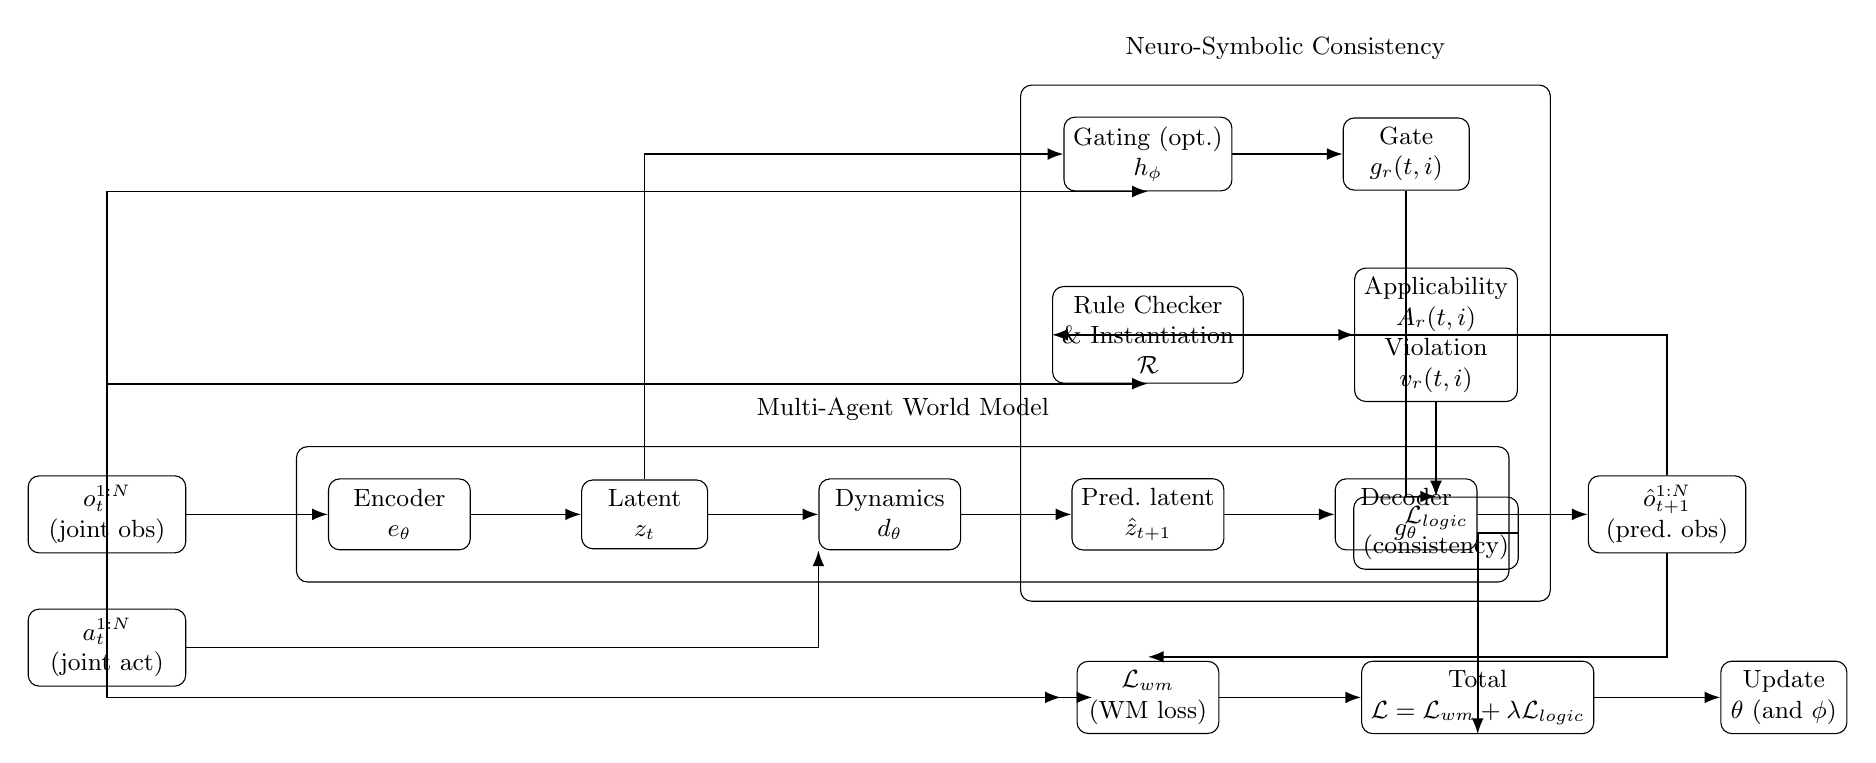
\begin{tikzpicture}[
                font=\small,
                node distance=10mm and 14mm,
                box/.style={draw, rounded corners, align=center, minimum height=9mm, minimum width=18mm},
                smallbox/.style={draw, rounded corners, align=center, minimum height=8mm, minimum width=16mm},
                io/.style={draw, rounded corners, align=center, fill=white, minimum height=8mm, minimum width=20mm},
                loss/.style={draw, rounded corners, align=center, minimum height=9mm, minimum width=18mm},
                group/.style={draw, rounded corners, inner sep=4mm},
                arr/.style={-Latex, line width=0.6pt}
            ]

            % ====== Main WM pipeline ======
            \node[io] (obs) {$o_t^{1:N}$\\(joint obs)};
            \node[io, below=7mm of obs] (act) {$a_t^{1:N}$\\(joint act)};

            \node[box, right=18mm of obs] (enc) {Encoder\\$e_\theta$};
            \node[smallbox, right=14mm of enc] (zt) {Latent\\$z_t$};

            \node[box, right=14mm of zt] (dyn) {Dynamics\\$d_\theta$};
            \node[smallbox, right=14mm of dyn] (znext) {Pred.\ latent\\$\hat z_{t+1}$};

            \node[box, right=14mm of znext] (dec) {Decoder\\$g_\theta$};
            \node[io, right=14mm of dec] (opred) {$\hat o_{t+1}^{1:N}$\\(pred.\ obs)};

            % arrows main
            \draw[arr] (obs) -- (enc);
            \draw[arr] (enc) -- (zt);
            \draw[arr] (zt) -- (dyn);
            \draw[arr] (dyn) -- (znext);
            \draw[arr] (znext) -- (dec);
            \draw[arr] (dec) -- (opred);

            % action into dynamics
            \draw[arr] (act) -| (dyn.south west);

            % ====== Losses ======
            \node[loss, below=14mm of znext] (lwm) {$\mathcal{L}_{wm}$\\(WM loss)};
            \draw[arr] (opred.south) |- ($(lwm.north)+(0,0.5mm)$);
            \draw[arr] (obs.south)  |- ($(lwm.west)+(-2mm,0)$); % indicates supervision / target
            \draw[arr] (act.south)  |- ($(lwm.west)+(2mm,0)$);

            % ====== Neuro-symbolic constraint path ======
            \node[box, above=12mm of znext] (rules) {Rule Checker\\\& Instantiation\\$\mathcal{R}$};
            \node[smallbox, right=14mm of rules] (viol) {Applicability\\$A_r(t,i)$\\Violation\\$v_r(t,i)$};

            \draw[arr] (opred.north) |- (rules.west);
            \draw[arr] (act.north)  |- (rules.south);
            \draw[arr] (rules) -- (viol);

            % gating (optional)
            \node[box, above=12mm of rules] (gate) {Gating (opt.)\\$h_\phi$};
            \node[smallbox, right=14mm of gate] (gcoef) {Gate\\$g_r(t,i)$};

            \draw[arr] (zt.north) |- (gate.west);
            \draw[arr] (act.north) |- (gate.south);
            \draw[arr] (gate) -- (gcoef);

            % logic loss
            \node[loss, below=12mm of viol] (llogic) {$\mathcal{L}_{logic}$\\(consistency)};
            \draw[arr] (viol) -- (llogic);
            \draw[arr] (gcoef) |- (llogic.north);

            % total objective
            \node[loss, right=18mm of lwm] (ltot) {Total\\$\mathcal{L}=\mathcal{L}_{wm}+\lambda\mathcal{L}_{logic}$};
            \draw[arr] (lwm) -- (ltot);
            \draw[arr] (llogic) -| (ltot.south);

            % parameter update annotation
            \node[smallbox, right=16mm of ltot] (upd) {Update\\$\theta$ (and $\phi$)};
            \draw[arr] (ltot) -- (upd);

            % ====== Group boxes (optional, for readability) ======
            \node[group, fit=(enc)(zt)(dyn)(znext)(dec), label={[yshift=2mm]above:Multi-Agent World Model}] (wmgroup) {};
            \node[group, fit=(rules)(viol)(gate)(gcoef)(llogic), label={[yshift=2mm]above:Neuro-Symbolic Consistency}] (nsgroup) {};

        \end{tikzpicture}}

    \caption{Overview of NS-MAWM. A multi-agent world model encodes joint observations, predicts latent dynamics conditioned on joint actions, and decodes predicted observations. Neuro-symbolic rules are instantiated on predictions to compute applicability and violation scores; an optional gating network modulates rule enforcement. Training minimizes $\mathcal{L}_{wm} + \lambda \mathcal{L}_{logic}$.}
    \label{fig:overview}
\end{figure}


\subsection{Structured observation latent space and unified neuro-symbolic formalism}
\label{sec:ns}

TODO

\subsection{The three neuro-symbolic integration strategies}
\label{sec:integration_strategies}

\subsubsection{The symbolic loss regularization strategy}
\label{sec:symbolic_loss_regularization}

TODO

\subsubsection{The symbolic projection strategy}
\label{sec:symbolic_projection}

TODO

\subsubsection{The residual symbolic dynamics strategy}
\label{sec:residual_symbolic_dynamics}

TODO

\subsection{Rule Violation Rate (RVR)}
\label{sec:rvr}

TODO

\subsection{NS-MAWM global algorithm}
\label{sec:algo}

TODO

% ============================
\section{Evaluation}
\label{sec:eval}

This section evaluates whether enforcing neuro-symbolic consistency in multi-agent world models effectively reduces semantic drift, improves long-horizon prediction fidelity, and benefits downstream decision-making.
Our evaluation protocol is explicitly designed to address the four gaps identified in the Introduction:
(G1) semantic invariants,
(G2) action-conditioned equivariances,
(G3) uncertainty-aware constraint application,
and (G4) semantic evaluation of world models.

\subsection{Environments}
\label{sec:envs}

We consider two classes of environments: a controlled grid-based multi-agent environment designed to precisely test semantic consistency, and a standard multi-agent benchmark to assess scalability and downstream impact.

\paragraph{Gridworld with Objects and Multiple Agents.}
We introduce a configurable gridworld environment in which $N\in\{2,3,4\}$ agents interact with static and dynamic objects placed on a discrete 2D grid.
Each cell may contain at most one object and at most one agent.
Agents perceive only a local $k\times k$ observation window centered on their position (with $k=3$ unless otherwise specified), inducing partial observability.
Observations are represented as multi-channel tensors encoding object types, agent presence, and free space.

Agents can execute primitive actions (move up/down/left/right, no-op), which induce deterministic or stochastic transitions depending on the experimental setting.
Crucially, this environment admits a rich set of semantic invariants and equivariances, including:
(i) object permanence,
(ii) spatial translation consistency under agent motion,
(iii) exclusivity constraints (no overlapping objects),
and (iv) conservation of object count.
These properties make the environment particularly suitable for studying semantic drift in learned world models.

We vary map sizes ($10\times10$ to $20\times20$), number of agents, object densities, and observability radii to systematically test generalization.
Out-of-distribution (OOD) evaluation is performed by increasing map size and object count at test time.

\paragraph{Standard Multi-Agent Benchmark.}
To assess whether improved world model consistency translates to realistic multi-agent domains, we additionally evaluate on a standard MARL benchmark with partial observability and coordination requirements.
We use a grid-based cooperative benchmark inspired by Overcooked-style layouts, where agents must coordinate to reach shared goals while observing only local information.
This benchmark is widely used in the MARL literature and provides a non-trivial test of scalability and robustness.

For this benchmark, the world model is trained on logged trajectories generated by a pretrained policy, and is evaluated both as a predictive model and as a simulator for planning-based or imagination-augmented control.

\subsection{Metrics}
\label{sec:metrics}

We employ a comprehensive set of metrics designed to jointly evaluate predictive accuracy, semantic consistency, and downstream utility.

\paragraph{Prediction Error.}
We report standard prediction metrics for world models:
(i) one-step prediction error and
(ii) $H$-step rollout error for horizons $H\in\{5,10,25,50\}$.
For discrete grid observations, prediction error is measured using cross-entropy and accuracy; for continuous features, we report mean squared error.
These metrics allow comparison with prior work on world models and model-based MARL.

\paragraph{Rule Violation Rate (RVR).}
To explicitly evaluate semantic correctness (G4), we introduce the \emph{Rule Violation Rate (RVR)}.
For a rollout of length $H$, RVR is defined as the average fraction of violated rules across agents and timesteps:
\[
  \mathrm{RVR}(H) = \frac{1}{H N |\mathcal{R}|}
  \sum_{t=1}^{H}\sum_{i=1}^{N}\sum_{r\in\mathcal{R}}
  \mathbb{I}\big[v_r(t,i) > 0\big].
\]
We also report a \emph{Soft-RVR}, which averages the continuous violation scores $v_r(t,i)$ and captures violation severity.

\paragraph{Long-Horizon Semantic Drift Curves.}
To visualize error accumulation, we report RVR as a function of rollout horizon $H$.
These curves directly quantify semantic drift and allow fine-grained comparison between models with similar predictive accuracy but different long-horizon behavior.

\paragraph{Downstream Control Performance.}
When the world model is used for planning or imagination-based policy learning, we additionally report:
(i) episodic return,
(ii) success rate,
and (iii) data efficiency (return versus number of environment interactions).
This evaluates whether improvements in world model consistency translate into practical benefits.

\subsection{Baselines}
\label{sec:baselines}

We compare NS-MAWM against a diverse set of baselines to isolate the effect of neuro-symbolic constraints.

\paragraph{Neural Multi-Agent World Model (MAWM).}
A purely neural world model with the same backbone architecture as NS-MAWM, trained using only $\mathcal{L}_{wm}$.
This baseline isolates the contribution of symbolic consistency.

\paragraph{Capacity-Controlled Baseline.}
To rule out gains due to increased model capacity, we include a neural MAWM with a larger latent dimension and deeper dynamics network, matched in parameter count to NS-MAWM.

\paragraph{Ablation Variants.}
We evaluate several ablations of our method:
(i) NS-MAWM without gating ($g_r \equiv 1$),
(ii) NS-MAWM with subsets of rules (e.g., invariants only or equivariances only),
(iii) varying the consistency weight $\lambda$,
and (iv) hard constraint variants where violations are projected rather than penalized (when applicable).

\paragraph{Structured and Object-Centric Models.}
When feasible, we compare against structured world models that incorporate relational or object-centric inductive biases but do not explicitly enforce symbolic constraints.
This assesses whether structure alone suffices to prevent semantic drift.

\subsection{Implementation Details}
\label{sec:impl}

All world models share the same backbone architecture unless otherwise specified.
Encoders and decoders are implemented as convolutional networks for grid observations, while dynamics models use either multilayer perceptrons or attention-based modules.
Latent dimensionality is set to $d=128$ by default.

Models are trained using Adam with learning rate $3\times10^{-4}$ and batch size 64.
Rule evaluation is vectorized across agents and rules, adding negligible overhead (less than 10\% additional computation per training step).
Training is performed on a single GPU; full training times range from 2 to 6 hours depending on environment size.

To ensure reproducibility, all experiments are run with 5 random seeds.
Hyperparameters are selected using a held-out validation set.
Code, environments, and rule specifications will be released upon publication.

\subsection{Results}
\label{sec:results}

\paragraph{Semantic Consistency and Long-Horizon Prediction.}
Table~\ref{tab:wm_consistency} summarizes prediction accuracy and semantic consistency for different world models on the gridworld benchmark.
All models achieve comparable one-step prediction accuracy, indicating that short-horizon predictive performance alone does not distinguish semantic quality.
However, as the rollout horizon increases, purely neural world models exhibit rapidly increasing semantic violations, reflected by sharply higher Rule Violation Rates (RVR).
In contrast, NS-MAWM maintains low violation rates even for long horizons ($H=50$), demonstrating substantially reduced semantic drift.

\begin{table}[t]
  \centering
  \small
  \setlength{\tabcolsep}{5pt}
  \begin{tabular}{lcccc}
    \toprule
    \textbf{Model}                  &
    \textbf{1-step CE $\downarrow$} &
    \textbf{RVR@10 $\downarrow$}    &
    \textbf{RVR@25 $\downarrow$}    &
    \textbf{RVR@50 $\downarrow$}                                                                     \\
    \midrule
    Neural MAWM
                                    & 0.183          & 0.21          & 0.38          & 0.57          \\
    Neural MAWM (large)
                                    & 0.176          & 0.19          & 0.34          & 0.52          \\
    Structured WM
                                    & 0.179          & 0.17          & 0.29          & 0.44          \\
    \midrule
    NS-MAWM (full)
                                    & \textbf{0.175} & \textbf{0.07} & \textbf{0.10} & \textbf{0.14} \\
    \bottomrule
  \end{tabular}
  \caption{Prediction accuracy and semantic consistency on gridworld environments.
    CE denotes cross-entropy loss.
    RVR@H is the Rule Violation Rate after an $H$-step rollout.
    Lower is better ($\downarrow$).
  }
  \label{tab:wm_consistency}
\end{table}

\paragraph{Ablation Analysis.}
To isolate the contribution of different components, we report ablation results in Table~\ref{tab:ablation}.
Using only invariants or only equivariances significantly improves semantic consistency over the neural baseline, but neither is sufficient on its own.
Removing the gating mechanism increases violation rates in stochastic or partially observable settings, confirming the importance of uncertainty-aware constraint application (G3).
The full NS-MAWM model consistently achieves the best trade-off between flexibility and semantic correctness.

\begin{table}[t]
  \centering
  \small
  \setlength{\tabcolsep}{6pt}
  \begin{tabular}{lccc}
    \toprule
    \textbf{Variant}                  &
    \textbf{RVR@25 $\downarrow$}      &
    \textbf{Soft-RVR@25 $\downarrow$} &
    \textbf{1-step CE}                                                                 \\
    \midrule
    Neural MAWM
                                      & 0.38          & 0.44          & 0.183          \\
    + Invariants only
                                      & 0.21          & 0.26          & 0.181          \\
    + Equivariances only
                                      & 0.24          & 0.29          & 0.180          \\
    NS-MAWM w/o gating
                                      & 0.16          & 0.20          & 0.177          \\
    \midrule
    NS-MAWM (full)
                                      & \textbf{0.10} & \textbf{0.13} & \textbf{0.175} \\
    \bottomrule
  \end{tabular}
  \caption{Ablation study on semantic consistency.
    Soft-RVR averages continuous violation magnitudes.
  }
  \label{tab:ablation}
\end{table}

\paragraph{Downstream Performance.}
Table~\ref{tab:downstream} reports downstream control performance when world models are used for imagination-based planning or policy improvement.
Despite similar one-step prediction error, NS-MAWM yields higher episodic returns and better data efficiency.
Importantly, gains correlate more strongly with reduced RVR than with prediction loss, highlighting the central role of semantic consistency for effective planning.

\begin{table}[t]
  \centering
  \small
  \setlength{\tabcolsep}{6pt}
  \begin{tabular}{lccc}
    \toprule
    \textbf{Model}                   &
    \textbf{Return $\uparrow$}       &
    \textbf{Success Rate $\uparrow$} &
    \textbf{Samples to 80\% $\downarrow$}                                             \\
    \midrule
    Neural MAWM
                                     & 42.1          & 0.61          & 1.0M           \\
    Neural MAWM (large)
                                     & 44.3          & 0.64          & 0.9M           \\
    Structured WM
                                     & 46.7          & 0.68          & 0.8M           \\
    \midrule
    NS-MAWM (full)
                                     & \textbf{53.9} & \textbf{0.78} & \textbf{0.55M} \\
    \bottomrule
  \end{tabular}
  \caption{Downstream planning and control performance.
    Higher return and success rate are better ($\uparrow$);
    fewer samples indicate higher data efficiency ($\downarrow$).
  }
  \label{tab:downstream}
\end{table}

\paragraph{Qualitative Analysis.}
Qualitative rollouts corroborate the quantitative results.
Neural world models frequently hallucinate objects, violate exclusivity constraints, or break spatial coherence after a few steps.
In contrast, NS-MAWM preserves object permanence and spatial relations over long rollouts, producing trajectories that remain visually and semantically plausible.

Overall, these results demonstrate that neuro-symbolic consistency constraints substantially improve the reliability, interpretability, and downstream utility of multi-agent world models, especially in long-horizon and partially observable regimes.

% ============================
% 7. Conclusion
% ============================
\section{Conclusion and future work}
\label{sec:conclusion}

This paper addressed a fundamental limitation of multi-agent world models: while neural world models can achieve strong short-horizon prediction accuracy, they often fail to preserve semantic consistency under long-horizon rollouts, particularly in partially observable multi-agent settings.
We introduced \textbf{Neuro-Symbolic Multi-Agent World Models (NS-MAWM)}, a framework that integrates symbolic invariants and action-conditioned equivariances as soft, differentiable consistency constraints during world model training.
By treating symbolic knowledge as an inductive bias rather than a hard restriction, NS-MAWM reduces semantic drift while preserving uncertainty and flexibility.

Empirically, we demonstrated that NS-MAWM substantially improves long-horizon semantic consistency, as measured by the proposed Rule Violation Rate (RVR), while maintaining comparable one-step predictive accuracy.
Across controlled gridworld environments and a standard multi-agent benchmark, these improvements translated into more reliable imagination rollouts, improved downstream planning performance, and higher data efficiency.
Ablation studies further showed that both invariants and equivariances contribute to performance, and that uncertainty-aware gating is critical in stochastic or partially observable regimes.

Beyond the specific instantiation presented in this work, NS-MAWM opens several promising research directions.
First, richer rule languages could be explored, including relational, temporal, or probabilistic rules that capture higher-level interaction patterns.
Second, while we focused on soft consistency constraints, investigating hybrid approaches that combine soft regularization with occasional hard projection or constraint satisfaction may further improve robustness.
Third, evaluating neuro-symbolic world models in more complex environments—such as continuous control, heterogeneous agent populations, or large-scale coordination tasks—remains an important step toward real-world applicability.

Another key direction concerns the source and reliability of symbolic knowledge.
In this work, rules were specified manually, which is appropriate for controlled settings but may not scale.
Future work could explore learning rules directly from data, combining representation learning with structure discovery, or adapting rules online as the environment changes.
Handling partial, incorrect, or conflicting rules, as well as stochastic events that temporarily violate invariants, is another important challenge.
The proposed gating mechanism is a first step in this direction, but more principled uncertainty-aware or Bayesian treatments are worth exploring.

Finally, scalability and transfer remain open questions.
As the number of agents or rules increases, efficient rule evaluation and selection becomes critical.
Investigating modular rule sets, rule sharing across agents, and transfer of learned constraints across domains may significantly broaden the applicability of neuro-symbolic world models.

\paragraph{Take-home message.}
Semantic consistency is a first-class requirement for reliable multi-agent world models.
By integrating neuro-symbolic consistency constraints into model-based MARL, NS-MAWM provides a principled and effective way to reduce long-horizon drift, improve interpretability, and enhance downstream decision-making.
We hope this work encourages further research at the intersection of world modeling, multi-agent systems, and neuro-symbolic learning.


\section*{Impact Statement}

This paper presents work whose goal is to advance the field of Machine Learning by improving the reliability of model-based multi-agent reinforcement learning.
By reducing semantic inconsistencies in learned world models, this work may contribute to safer and more interpretable decision-making in multi-agent systems.
We do not identify ethical concerns specific to this work beyond those commonly associated with reinforcement learning research.


% ============================
% Acknowledgements (remove for submission if needed)
% ============================
% \section*{Acknowledgements}

% ============================
% References
% ============================
\bibliography{references}
\bibliographystyle{icml2026}

%%%%%%%%%%%%%%%%%%%%%%%%%%%%%%%%%%%%%%%%%%%%%%%%%%%%%%%%%%%%%%%%%%%%%%%%%%%%%%%
%%%%%%%%%%%%%%%%%%%%%%%%%%%%%%%%%%%%%%%%%%%%%%%%%%%%%%%%%%%%%%%%%%%%%%%%%%%%%%%
% APPENDIX
%%%%%%%%%%%%%%%%%%%%%%%%%%%%%%%%%%%%%%%%%%%%%%%%%%%%%%%%%%%%%%%%%%%%%%%%%%%%%%%
%%%%%%%%%%%%%%%%%%%%%%%%%%%%%%%%%%%%%%%%%%%%%%%%%%%%%%%%%%%%%%%%%%%%%%%%%%%%%%%

\newpage

\appendix

\section{Rule Set Details}
\label{app:rules}
% TODO:
% - list rules formally
% - applicability masks
% - examples

\section{Additional Experimental Results}
\label{app:more}
% TODO:
% - ablations, extra environments, hyperparams

\section{Architectures and Hyperparameters}
\label{app:hparams}
% TODO:
% - full hyperparam tables

%%%%%%%%%%%%%%%%%%%%%%%%%%%%%%%%%%%%%%%%%%%%%%%%%%%%%%%%%%%%%%%%%%%%%%%%%%%%%%%
%%%%%%%%%%%%%%%%%%%%%%%%%%%%%%%%%%%%%%%%%%%%%%%%%%%%%%%%%%%%%%%%%%%%%%%%%%%%%%%

\end{document}

% This document was modified from the file originally made available by
% Pat Langley and Andrea Danyluk for ICML-2K. This version was created
% by Iain Murray in 2018, and modified by Alexandre Bouchard in
% 2019 and 2021 and by Csaba Szepesvari, Gang Niu and Sivan Sabato in 2022.
% Modified again in 2023 and 2024 by Sivan Sabato and Jonathan Scarlett.
% Previous contributors include Dan Roy, Lise Getoor and Tobias
% Scheffer, which was slightly modified from the 2010 version by
% Thorsten Joachims & Johannes Fuernkranz, slightly modified from the
% 2009 version by Kiri Wagstaff and Sam Roweis's 2008 version, which is
% slightly modified from Prasad Tadepalli's 2007 version which is a
% lightly changed version of the previous year's version by Andrew
% Moore, which was in turn edited from those of Kristian Kersting and
% Codrina Lauth. Alex Smola contributed to the algorithmic style files.
